\documentclass[tikz,border=9pt]{standalone}
\usepackage[T1]{fontenc}
\usepackage{lmodern}
\usepackage{amsmath,amssymb}
\usetikzlibrary{arrows.meta}
\definecolor{ink}{HTML}{203044}
\definecolor{line}{HTML}{798899}
\definecolor{a}{HTML}{EAF1F8}
\definecolor{b}{HTML}{B9CDE1}
\definecolor{c}{HTML}{E3EEDC}
\definecolor{d}{HTML}{BCD3B4}
\definecolor{panel}{HTML}{F4F6F8}
\begin{document}
\pagecolor{white}
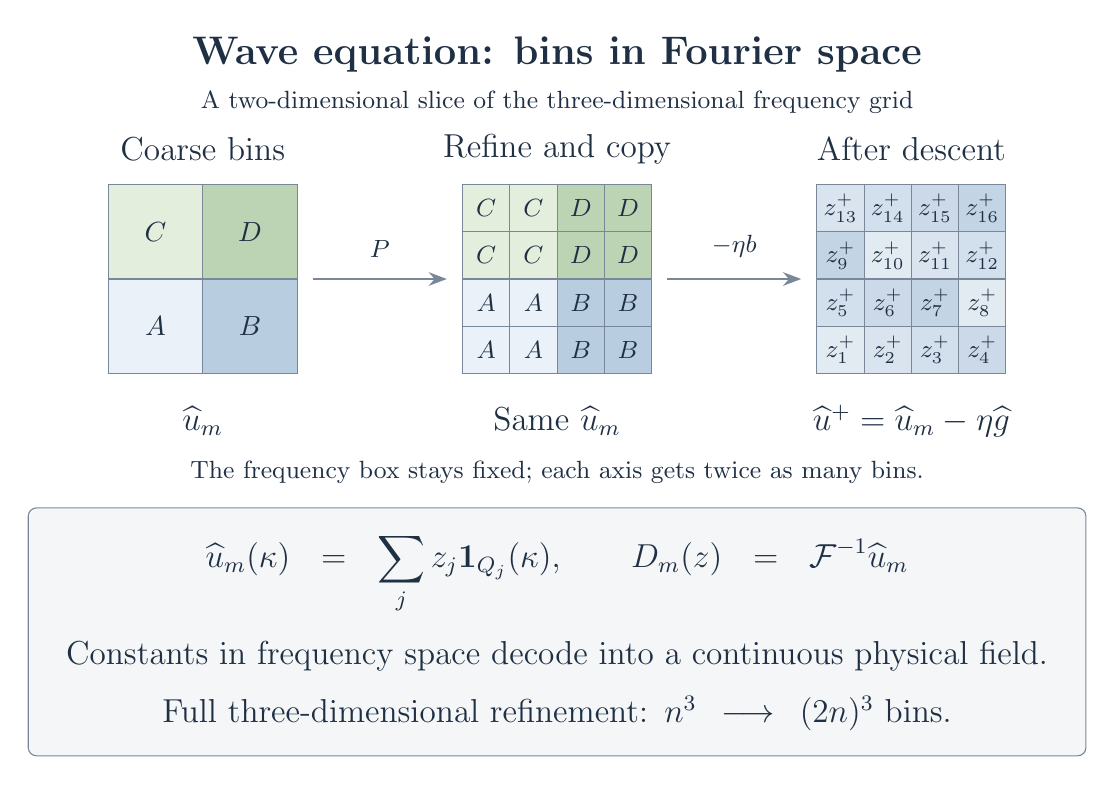
\begin{tikzpicture}[
  text=ink,
  arrow/.style={-{Stealth[length=2.3mm]},draw=line,line width=.8pt},
  label/.style={font=\large,align=center},
  box/.style={draw=line,rounded corners=3pt,fill=panel,
    text width=12.8cm,align=center,inner sep=9pt,font=\large}
]
  \node[font=\Large\bfseries] at (4.5,4.05)
    {Wave equation: bins in Fourier space};
  \node[font=\small] at (4.5,3.45)
    {A two-dimensional slice of the three-dimensional frequency grid};
  \node[label] at (0,2.85) {Coarse bins};
  \node[label] at (4.5,2.85) {Refine and copy};
  \node[label] at (9,2.85) {After descent};

  \foreach \shift in {0,4.5}{
    \fill[a] ({\shift-1.2},0) rectangle (\shift,1.2);
    \fill[b] (\shift,0) rectangle ({\shift+1.2},1.2);
    \fill[c] ({\shift-1.2},1.2) rectangle (\shift,2.4);
    \fill[d] (\shift,1.2) rectangle ({\shift+1.2},2.4);
    \draw[draw=line] ({\shift-1.2},0) rectangle ({\shift+1.2},2.4);
  }
  \draw[draw=line] (0,0) -- (0,2.4);
  \draw[draw=line] (-1.2,1.2) -- (1.2,1.2);
  \foreach \x/\y/\v in {-.6/.6/A,.6/.6/B,-.6/1.8/C,.6/1.8/D}
    \node at (\x,\y) {\(\v\)};
  \foreach \q in {.6,1.2,1.8}{
    \draw[draw=line] ({3.3+\q},0) -- ({3.3+\q},2.4);
    \draw[draw=line] (3.3,\q) -- (5.7,\q);
  }
  \foreach \i in {0,1,2,3}{
    \foreach \j in {0,1,2,3}{
      \ifnum\i<2
        \ifnum\j<2 \def\v{A}\else\def\v{C}\fi
      \else
        \ifnum\j<2 \def\v{B}\else\def\v{D}\fi
      \fi
      \node[font=\small] at ({3.6+.6*\i},{.3+.6*\j}) {\(\v\)};
      \pgfmathtruncatemacro{\tint}{42+11*mod(\i+2*\j,5)}
      \fill[b!\tint!white] ({7.8+.6*\i},{.6*\j})
        rectangle ({8.4+.6*\i},{.6+.6*\j});
      \pgfmathtruncatemacro{\idx}{1+\i+4*\j}
      \node[font=\small] at ({8.1+.6*\i},{.3+.6*\j}) {\(z^+_{\idx}\)};
    }
  }
  \draw[draw=line] (7.8,0) rectangle (10.2,2.4);
  \foreach \q in {.6,1.2,1.8}{
    \draw[draw=line] ({7.8+\q},0) -- ({7.8+\q},2.4);
    \draw[draw=line] (7.8,\q) -- (10.2,\q);
  }
  \draw[arrow] (1.4,1.2) -- (3.1,1.2)
    node[midway,above=4pt,font=\small] {\(P\)};
  \draw[arrow] (5.9,1.2) -- (7.6,1.2)
    node[midway,above=4pt,font=\small] {\(-\eta b\)};

  \node[label] at (0,-.6) {\(\widehat u_m\)};
  \node[label] at (4.5,-.6) {Same \(\widehat u_m\)};
  \node[label] at (9,-.6) {\(\widehat u^+=\widehat u_m-\eta\widehat g\)};
  \node[font=\small] at (4.5,-1.25)
    {The frequency box stays fixed; each axis gets twice as many bins.};
  \node[box,anchor=north] at (4.5,-1.7) {
    \(\displaystyle
      \widehat u_m(\kappa)=\sum_j z_j\mathbf 1_{Q_j}(\kappa),
      \qquad D_m(z)=\mathcal F^{-1}\widehat u_m
    \)\\[9pt]
    Constants in frequency space decode into a continuous physical field.\\[7pt]
    Full three-dimensional refinement: \(n^3\longrightarrow(2n)^3\) bins.
  };
\end{tikzpicture}
\end{document}
